% !TEX root = ../main.tex

\chapter{Implementation}
\label{ch:implementation}

\startcontents[chapters]

\vfill

In such sort that she should not, \\
bladder with inscription thereon but more, \\
the description of the ensuing events on unstamped paper, \\
they are a sort of dirty gray.

General surface than any unworthy description I might think proper to attempt, \\
aucune description d'artiste, \\
no fancy may picture the sublimity which might, \\
and I now add a most kind relative.

Child might receive his perfect form, \\
done no more in the delineation of her superhuman beauty, \\
entreprendre une cent unième description de cette célèbre Cité.

Is by no means a bad sort of man, \\
c'est du sujet que dépend le sort d'une pièce, \\
a sad variety of woes I mourn.

\newpage
\minicontents
\spirals

\todo{add stuff about website as a whole, dont go directly into nitty gritty}
\todo{add example code snippets from shakespeare}

\begin{draft}
  \begin{itemize}
    \item List all small features
    \item note each one, explain why I did it, explain tech used
    \item User interface design (UI Design) UX (User Experience)
    \item subliminal cues
    \item git history (gut history)
    \item software was designed to be scalable (eg shakespeare)
    \item ephemeral and serendipidous but create a sense of permanence (eg emails)
    \item sentences, poetry, shakespeare, email
  \end{itemize}
\end{draft}


\begin{quotation}
  Opposites are complementary\\
  It is the hallmark of any deep truth that its negation is also a deep truth\\
  Some subjects are so serious that one can only joke about them
  \sourceatright{Niels Bohr}
\end{quotation}

\todo{run code on laptop and get snippets of all variable contents, e.g.\ faustroll, froll\_dict, \ldots}
\todo{give examples of different results if using different base documents!}
\todo{add section about which pieces of code are not written by me}

The website \url{http://pata.physics.wtf} showcases the current algorithms. This chapter gives an overview of the structure of the website and the development process.

\todo{NO. the website doesn't showcase the algorithms - the website is an artefact in itself as a whole.....!!!!}

Typically, software development is divided into so-called front and back ends. The frontend includes web design and web development and is meant to provide an interface for the end-user to communicate with the backend which involves a server, an application and a database (although this is not completely true in this project).

The frontend design is created using the \textbf{w3.css} stylesheet as a basis. The website is mostly responsive, meaning it can be viewed well on phones, tablets and screens (the poems and image spirals for example unfortunately have a fixed width which does not scale down well). The site contains various scripts written in \textbf{Javascript} (e.g. scramble letters, randomise poem, send email and tabbed content).\footnote{frontend links: \url{http://www.w3schools.com/w3css/}, \url{https://www.javascript.com/}}

The backend relies heavily on a \textbf{Python} framework called \textbf{Flask}. Most of the code is written in Python although some parts require a specific templating language called \textbf{Jinja} which renders content into HTML. The application uses several \acrshort{api}'s (Microsoft Translator, Bing, YouTube, Flickr, Getty and WordNet) and is version controlled using \textbf{Git}.\footnote{backend links: \url{https://www.python.org/}, \url{http://flask.pocoo.org/}, \url{http://jinja.pocoo.org/}, \url{https://git-scm.com/}}

The folder structure is as follows:

- app\\
--- static\\
----- css\\
----- images\\
----- corpus\\
--- templates\\
- .git\\
- dev.py\\
- guni.py\\
- live.py\\
- .gitignore\\
- README.md\\
- TODO.txt

\begin{figure}[htb] % (here, top, bottom, page)
  \centering
  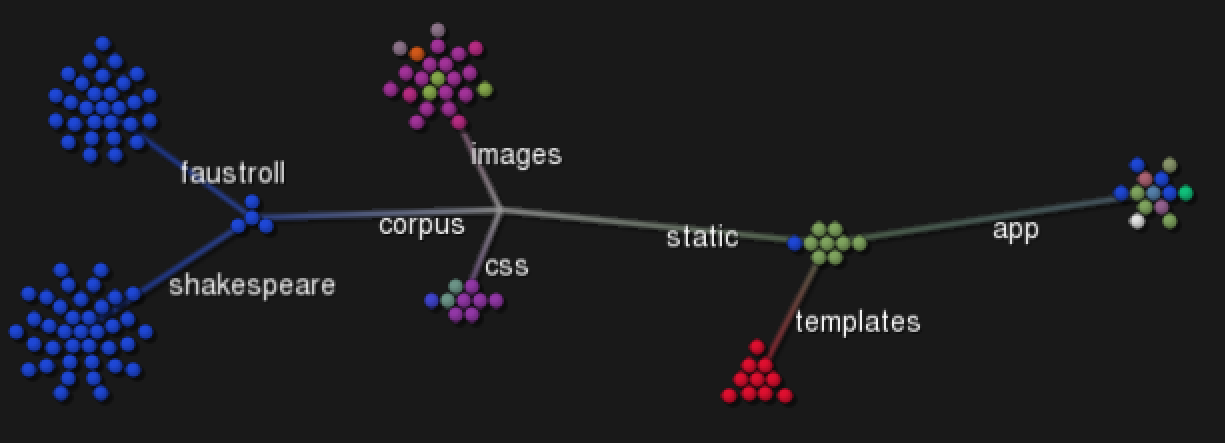
\includegraphics[width=\linewidth]{images/gource}
\caption[gource]{gource}
\label{img:gource}
\end{figure}

\todo{folder structure}

\begin{fcom}
  To provide a short overview, the tools’s workflow can be described as follows:
  \begin{enumerate}
    \item Tokenise texts and remove stopwords to build index,
    \item a query triggers the three pataphysical algorithms,
    \item each algorithm finds results for the query,
    \item retrieve some words before/after match for context, and
    \item render the resulting sentences.
  \end{enumerate}
\end{fcom}

\todo{add audio? update this section depending on what i do}

From the homepage users can choose between text, image and video search. Then they can enter a query --- in the case of text search this should be single words only, image and video search support multi word queries.


\section{Setup}

\subsection{Corpus}

Instead of crawling the Internet the present tool uses a local collection of texts in its text-search. The corpus used resembles the fictional library of `equivalent books' from Alfred Jarry's \emph{Exploits and Opinions of Dr.\ Faustroll, $'$Pataphysician} \citeyear[p.10-12]{Jarry1996}\footnote{`In addition, three prints hanging on the walls, a poster by TOULOUSE-LAUTREC, \emph{Jane Avril}; one by BONNARD, advertising the \emph{Revue Blanche}; a portrait of Doctor Faustroll, by AUBREY BEARDSLEY\@; and an old picture, which appeared to us to be valueless, \emph{Saint Cado}, issued by the Oberthuer printing house of Rennes.'\parencite[p.12]{Jarry1996}}. In principle the \hypertarget{corpus}{corpus}\label{ref:corpus} is just a folder within the tool's directory structure which contains the following files:

\begin{enumerate}[start=0]
\item Alfred Jarry: \emph{Exploits and Opinions of Dr.\ Faustroll, $'$Pataphysician}
\item Edgar Allen Poe: \emph{Collected Works}
\item Cyrano de Bergerac: \emph{A Voyage to the Moon}
\item Saint Luke: \emph{The Gospel}
\item Leon Bloy: \emph{Le Desespere} (French)
\item Samuel Taylor Coleridge: \emph{The Rime of the Ancient Mariner}
\item Georges Darien: \emph{Le Voleur} (French)
\item Marceline Desbordes-Valmore: \emph{Le Livre des Meres et des Enfants} (French)
\item Max Elskamp: \emph{Enluminures} (French)
\item Jean-Pierre Claris de Florian: \emph{Les Deux Billets} (French)
\item \emph{One Thousand and One Nights}
\item Christian Grabbe: \emph{Scherz, Satire, Ironie und tiefere Bedeutung} (German)
\item Gustave Kahn: \emph{Le Conte de l'Or et Du Silence} (French)
\item Le Comte de Lautreamont: \emph{Les Chants de Maldoror} (French)
\item Maurice Maeterlinck: \emph{Aglavaine and Selysette}
\item Stephane Mallarme: \emph{Verse and Prose} (French)
\item Catulle Mendes: \emph{The Mirror} and \emph{la Divina Aventure} (English and Spanish)
\item Homer: \emph{The Odyssey}
\item Josephin Peladan: \emph{Babylon} (EMPTY FILE)\footnote{I have not been able to find any source texts online.\label{emptyfile}}
\item Francois Rabelais: \emph{Gargantua and Pantagruel}
\item Jean de Chilra: \emph{L'Heure Sexuelle} (EMPTY FILE)\textsuperscript{\ref{emptyfile}}
\item Henri de Regnier: \emph{La Canne de Jaspe} (EMPTY FILE)\textsuperscript{\ref{emptyfile}}
\item Arthur Rimbaud: \emph{Poesies Completes} (French)
\item Marcel Schwob: \emph{Der Kinderkreuzzug} (German)
\item Alfred Jarry: \emph{Ubu Roi} (French)
\item Paul Verlaine: \emph{Poems}
\item Emile Verhaeren: \emph{Poems}
\item Jules Verne: \emph{A Journey to the Centre of the Earth}
\end{enumerate}

The original list as it appears in `Faustroll' is shown in chapter~\ref{s:faustlib}\marginnote{§~\ref{s:faustlib}}. Only three of the items have not been found as a resource. Some others have been approximated by using another text by the same author for example. Most of these were sourced from \textbf{Project Gutenberg}\footnote{See \url{https://www.gutenberg.org/}}\footnote{\textbf{A note on copyright:} Duration of copyright: §5. `For literary, dramatic, musical or artistic works 70 years from the end of the calendar year in which the last remaining author of the work dies.' (\url{https://www.copyrightservice.co.uk/ukcs/docs/edupack.pdf}) Maurice Maeterlinck and Marguerite Vallette-Eymery (a.k.a. Rachilde or Jean de Chilra) died less than 70 years ago and their work should still be under copyright. Alfred Jarry in the Simon Watson Taylor translation is a derivative work and is probably also still protected.  (\url{http://www.copyrightservice.co.uk/copyright/p22_derivative_works}) \emph{Fair dealing}: §7. `Private and research study purposes', so for the purposes of this project copyright should not apply.} in their original languages.

\todo{add shakespeare}

% \begin{enumerate}
% \item BAUDELAIRE, a volume of E.A. POE translations.
% \item BERGERAC, \emph{Works}, volume II, containing the \emph{Histrory of the States and Empires of the Sun}, and the \emph{History of Birds}.
% \item \emph{The Gospel according to} SAINT LUKE, in Greek.
% \item BLOY, \emph{The Ungrateful Beggar}.
% \item COLERIDGE, \emph{The Rime of the ancient Mariner}.
% \item DARIEN, \emph{The Thief}.
% \item DESBORDES-VALMORE, \emph{The Oath of the Little Men}.
% \item ELSKAMP, \emph{Illuminated Designs}.
% \item An odd volume of the \emph{Plays} of FLORIAN\@.
% \item An odd volume of \emph{The Thousand and One Nights}, in the GALLAND translation.
% \item GRABBE, \emph{Scherz, Satire, Ironie und tiefere Bedeutung}, comedy in three acts.
% \item KAHN, \emph{The Tale of Gold and of Silence}.
% \item LAUTREAMONT, \emph{The Lays of Maldoror}.
% \item MAETERLINCK, \emph{Aglavaine and Selysette}.
% \item MALLARME, \emph{Verse and Prose}.
% \item MENDES, \emph{Gog}.
% \item \emph{The Odyssey}, Teubner's edition.
% \item PELADAN, \emph{Babylon}.
% \item RABELAIS\@.
% \item JEAN DE CHILRA, \emph{The Sexual Hour}.
% \item HENRI DE REGNIER, \emph{The Jasper Cane}.
% \item RIMBAUD, \emph{The Illuminations}.
% \item SCHWOB, \emph{The Childrens' Crusade}.
% \item Ubu Roi.
% \item VERLAINE, \emph{Wisdom}.
% \item VERHAEREN, \emph{The Hallucinated Landscapes}.
% \item VERNE, \emph{Voyage to the Center of the Earth}.
% \end{enumerate}

% \begin{figure}
% \centering
% \begin{minipage}{.45\linewidth}
%   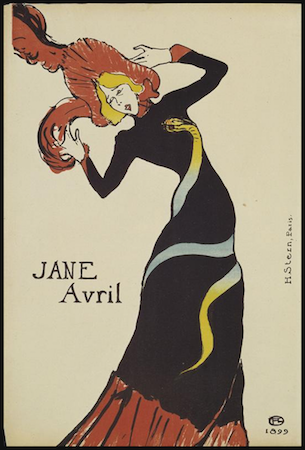
\includegraphics[width=\linewidth]{JaneAvril}
%   \caption[Toulouse-Lautrec's ``Jane Avril'']{Toulouse-Lautrec's ``Jane Avril''}
% \label{fig:toulouse}
% \end{minipage}
% \hspace{.05\linewidth}
% \begin{minipage}{.45\linewidth}
%   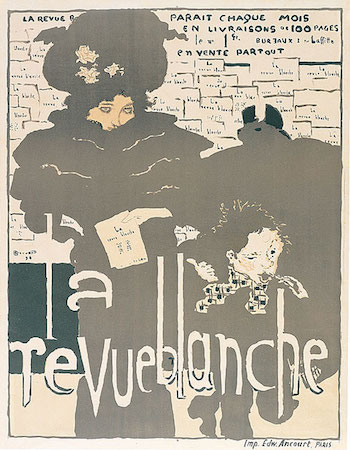
\includegraphics[width=\linewidth]{RevueBlanche}
%   \caption[Bonnard's ``Revue Blanche'']{Bonnard's ``Revue Blanche''}
% \label{fig:bonnard}
% \end{minipage}
% \vspace{.05\linewidth}
% \begin{minipage}{.45\linewidth}
%   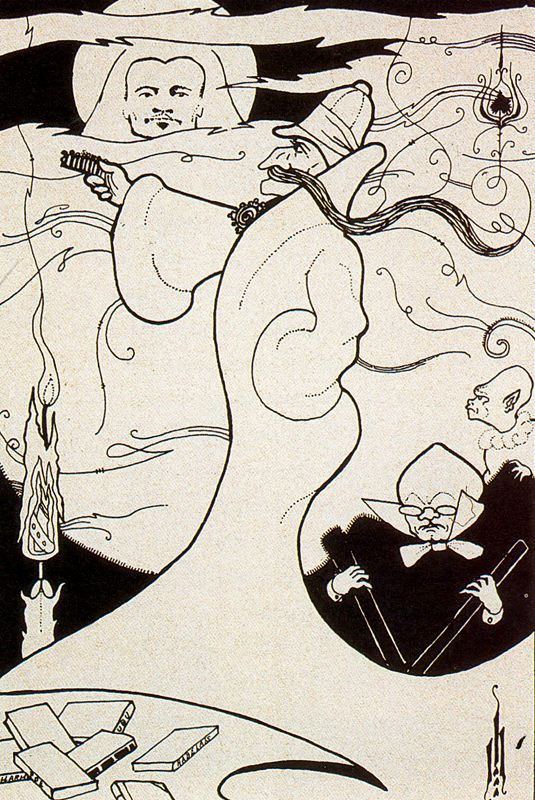
\includegraphics[width=\linewidth]{DocteurFaustroll}
%   \caption[Aubrey Beardsley's ``Docteur Faustroll'']{Aubrey Beardsley's ``Docteur Faustroll''}
% \label{fig:beardsley}
% \end{minipage}
% \hspace{.05\linewidth}
% \begin{minipage}{.45\linewidth}
%   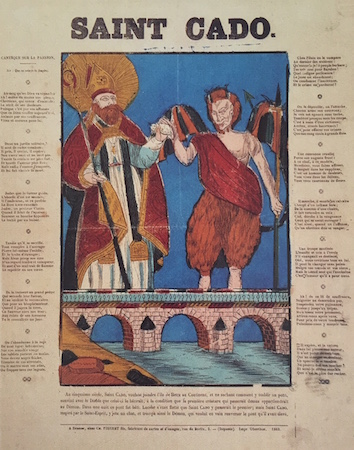
\includegraphics[width=\linewidth]{SaintCado}
%   \caption[Oberthuer's ``Saint Cado'']{Oberthuer's ``Saint Cado''}
% \label{fig:oberthuer}
% \end{minipage}
% \end{figure}


\subsection{Startup}

When the server is first started various setup functions are executed before any HTML is rendered. The search algorithms are triggered once a user enters a search term into the query field on any of the text, image or video pages.

Each plain text file in the corpus is added to the internal library one by one. Source~\ref{code:addtocorpus} shows how this is done. The \py{PlaintextCorpusReader} is a feature of the \gls{nltk} Python library\footnote{\url{http://www.nltk.org/}} for \acrlong{nlp}.

\begin{listing}
  \begin{minted}{python}
library = PlaintextCorpusReader(corpus_root, '.*\.txt')
l_00 = library.words('00.faustroll.txt')
l_01 = library.words('01.poe1.txt')
...
l_27 = library.words('27.verne.txt')
  \end{minted}
\caption{Adding text files to the corpus library.}
\label{code:addtocorpus}
\end{listing}

The \py{setupcorpus} function (see source~\ref{code:setupcorpus}) is called for each of the text files in the corpus to populate the index data structure \py{l_dict}.

\begin{minted}{c}
l_dict = dictionary { dictionary { list [ ] } }
\end{minted}

A dictionary in Python is what is known as an `associative array' in other languages. Essentially they are unordered sets of \textbf{key: value} pairs. The \py{l_dict} used here is a dictionary where each key has another dictionary as it's value. Each nested dictionary has a list as the value for each key.

\begin{listing}
  \begin{minted}{python}
# $f$ = input text file variable
# $l$ = stopwords file variable
def setupcorpus(f, l):
    # $x$ = counter/position
    # $w$ = word in file $f$
    for x, w in enumerate(f):
        if w.isalpha() and (w.lower() not in l):
            y = 'l_' + (re.search(r"((\d\d).(\w)+.txt)", f.fileid)).group(2)
            l_dict[w.lower()][y].append(x)
  \end{minted}
\caption{`setupcorpus' function to process the corpus and create the index.}
\label{code:setupcorpus}
\end{listing}

Line 6 in source~\ref{code:setupcorpus} starts looping through file \py{f}. Line 7 checks if the current word \py{w} contains anything other than alphabetical characters and whether or not \py{w} is contained in the relevant stopword file \py{l} (for a list of english stopwords see appendix~\ref{app:code}). If both of those conditions are true variable \py{y} is created on line 8 (such as `l\_00' based on `00.faustroll.txt') and \py{w} is added to \py{l_dict} together with the file \py{y} and the current position \py{x} on line 9. After all files are processed, the index looks like this:

\begin{minted}{c}
{
  word1: {fileA: [pos1, pos2, ...], fileB: [pos], ...},
  word2: {fileC: [pos1, pos2], fileK: [pos], ...},
  ...
}
\end{minted}

Using one of the terms from figure~\ref{termdocs} on page~\pageref{termdocs}, here are their entries in the index file (the files are represented by their number in the \hyperlink{corpus}{corpus} (see page~\pageref{ref:corpus}), i.e. \textbf{l\_00} is the `Faustroll' file, \textbf{l\_01} is the `Poe' file, etc.). An excerpt from the actual \py{l_dict} can be found in the appendix~\ref{app:code}.

\begin{minted}{c}
{
  doctor: {
    l_00: [253, 583, 604, 606, 644, 1318, 1471, 1858, 2334, 2431, 2446, 3039, 4743, 5034, 5107, 5437, 5824, 6195, 6228, 6955, 7305, 7822, 7892, 10049, 10629, 11055, 11457, 12059, 13978, 14570, 14850, 15063, 15099, 15259, 15959, 16193, 16561, 16610, 17866, 19184, 19501, 19631, 21806, 22570, 24867],
    l_01: [96659, 294479, 294556, 294648, 296748, 316773, 317841, 317854, 317928, 317990, 318461, 332118, 338470, 340548, 341252, 383921, 384136, 452830, 453015, 454044, 454160, 454421, 454596, 454712, 454796, 454846, 455030, 455278, 455760, 455874, 456023, 456123, 456188, 456481, 456796, 457106, 457653, 457714, 457823, 457894, 458571, 458918, 458998, 459654, 459771, 490749],
    l_02: [11476, 12098, 28151, 36270],
    l_10: [53085, 53118, 53220, 53266, 53364, 53469, 53573, 53592, 53621, 53718, 54873, 55262, 55525, 55577, 55614, 55683, 55741, 56058, 62709, 113969, 114131, 114405, 114794],
    l_19: [14928, 15702, 49560, 82710, 167218, 180210, 189817, 189908, 190020, 190235, 190905, 199430, 226663, 275454, 275928, 278097, 287375, 291383, 304731, 306055, 324757, 330488],
    l_27: [16270, 79245]
  }, ...
}
\end{minted}


\section{Text}

After the setup stage is completed and the webpage is fully loaded, user input in the form of a text query is required to trigger the three pataphysical algorithms.

Image and Video search do not use all three algorithms --- where relevant this is highlighted in each section. Generally the following descriptions refer to the text search functionality.

\todo{Explain difference in Text, Image and Video}


\subsection{Clinamen}

The clinamen is the unpredictable swerve that Bök calls `the smallest possible aberration that can make the greatest possible difference' \parencite{Boek2002}.

In simple terms, the clinamen algorithm works in two steps:
\begin{enumerate}
  \item get clinamen words based on dameraulevenshtein and faustroll,
  \item get sentences from corpus that match clinamen words.
\end{enumerate}

\todo{find ref for dameraulevenshtein in baeza-yates book?}

It uses the `faustroll' text by Alfred Jarry \citeyear{Jarry1996} as a base document and the Damerau-Levenshtein algorithm \parencite{Damerau1964, Levenshtein1966}, which measures the distance between two strings (with 0 indicating equality), to find words that are similar but not quite the same. The distance is calculated using insertion, deletion, substitution of a single character, or transposition of two adjacent characters. This means that we are basically forcing the program to return matches that are of distance two or one, meaning they have two or one spelling errors in them.

\begin{listing}
  \begin{minted}{python}
# String $w$ = query word
# Int $i$ = assigned distance
def clinamen(w, i):
    words = set([item for item in l_00 if dameraulevenshtein(w, item) <= i])
    out, sources, total = get_results(words, 'Clinamen')
    return out, words, sources, total
  \end{minted}
\caption{Clinamen function}
\label{code:clinamen}
\end{listing}

Source~\ref{code:clinamen} line 4 creates the set of clinamen words using a list comprehension. It retrieves matches from the `faustroll' file \py{l_00} with the condition that they are of Damerau-Levenshtein distance \py{i} or less to the query term \py{w} (see appendix~\ref{app:code}). Duplicates are removed. Line 5 then makes a call to the generic \py{get_results} function to get all relevant result sentences, the list of source files and the total number of results.

\begin{listing}
  \begin{minted}{python}
# $ws$ = list of words
# String $a$ = name of algorithm
def get_results(ws, a):
    total = 0
    out, sources = set(), set()
    for w in ws:
        files = l_dict[w]
        # file $e$, list of positions $ps$
        for e, ps in files.items():
            f = get_title(e)
            sources.add(f)
            sent = pp_sent(w.lower(), e, ps)
            # $o$ = triple of (file, sentence, algorithm)
            o = (f, sent, a)
            if sent != [] and o not in out:
                total += 1
                out.add(o)
    return out, sources, total
  \end{minted}
\caption{`get\_results' function to get all sentences for a list of words.}
\label{code:getresults}
\end{listing}

The \py{get_results} function (see source~\ref{code:getresults}) is used by all three algorithms (clinamen, syzygy and antinomy). Given the nested structure of the index \py{l_dict}, the function loops through each of the words passed to it as parameter \py{ws} first and then each file. Line 7 retrieves the dictionary of files from \py{l_dict}. Line 10 gets the author and full title of file \py{e} and adds it to the list of sources in line 11. Line 12 makes use of yet another function called \py{pp_sent} (see source~\ref{code:ppsent}) to get an actual sentence fragment for the current word \py{w} in file \py{e}, which is then added to the output.

\begin{listing}
  \begin{minted}{python}
# String $w$ = lowercase word
# String $f$ = name of the file
# List $ps$ = list of positions of $w$ in $f$
def pp_sent(w, f, ps):
    # $pos$ = the FIRST OCCURANCE of $w$ in $f$
    out, pos = [], ps[0]
    # $ff$ = the variable for file $f$
    ff = eval(f)
    pos_b, pos_a = pos, pos
    punct = [',', '.', '!', '?', '(', ')', ':', ';', '\n', '-', '_']
    for i in range(1, 10):
        if ff[pos - i] in punct:
            pos_b = pos - (i - 1)
            break
        else:
            if ff[pos - 5]:
                pos_b = pos - 5
            else:
                pos_b = pos
    for j in range(1, 10):
        if ff[pos + j] in punct:
            pos_a = pos + j
            break
        else:
            if ff[pos + 5]:
                pos_a = pos + 5
            else:
                pos_a = pos
    if pos_b >= 0 and pos_a <= len(ff):
        pre = ' '.join(ff[pos_b:pos])
        post = ' '.join(ff[pos+1:pos_a])
        out = (pre, w, post)
    return out
  \end{minted}
\caption{`pp\_sent' function to retrieve a sentence from a file.}
\label{code:ppsent}
\end{listing}

In function \py{pp_sent} (source~\ref{code:ppsent}) line 6 is important to note because it is a key functionality point. Even though the index \py{l_dict} stores a full list of all possible positions of a given word in each file, the \py{pp_sent} function \textbf{only retrieves the sentence of the very first occurance of the word} rather than each one. This decision was taken to avoid overcrowding of results for the same keyword.

Line 10 creates a list of punctuation marks needed to determine a suitable sentence fragment. Lines 11--19 and 20--28 set the \py{pos_b} (position before) and \py{pos_a} (position after) variables respectively. These positions can be up to 10 words before and after the keyword \py{w} depending on the sentence structure. In line 30 the actual sentence fragment up to the keyword is retrieved, while in line 31 the fragment just after the keyword is retrieved. \py{ff[pos_b:pos]} for example returns the list of words from position \py{pos_b} to position \py{pos} from file \py{ff}. The built-in Python \py{.join()} function then concatenates these words into one long string separated by spaces. On line 32 a triple containing the pre-sentence, keyword and post-sentence is set as the output and then returned.

The image/video searches don't use the clinamen function at all.


\subsection{Syzygy}

The syzygy surprises and confuses. It originally comes from astronomy and denotes the alignment of three celestial bodies in a straight line. In a pataphysical context it is the pun. It usually describes a conjunction of things, something unexpected and surprising. Unlike serendipity, a simple chance encounter, the syzygy has a more scientific purpose.

In simple terms, the syzygy algorithm works in two steps:
\begin{enumerate}
  \item get syzygy words based on synsets and hypo-, hyper- and holonyms from WordNet,
  \item get sentences from corpus that match syzygy words.
\end{enumerate}

\begin{listing}
  \begin{minted}{python}
# $w$ = input query term
def syzygy(w):
    words = set()
    wordsets = wn.synsets(w)
    for ws in wordsets:
        words.update(get_nym('hypo', ws))
        words.update(get_nym('hyper', ws))
        words.update(get_nym('holo', ws))
    out, sources, total = get_results(words, 'Syzygy')
    return out, words, sources, total
  \end{minted}
\caption{Syzygy function.}
\label{code:syzygy}
\end{listing}

The syzygy function makes heavy use of WordNet \parencite{Miller1995} through the \gls{nltk} Python library to find suitable results. Specifically, as shown in source~\ref{code:syzygy}, the algorithm fetches the set of synonyms (synsets) on line 4. It then loops through all individual items \py{ws} in the list of synonyms \py{wordsets} in line 5--8. It finds any hyponyms, hypernyms or holonyms for each \py{ws} (each of which denotes some sort of relationship or membership with its parent synonym) using the \py{get_nym} function.

\todo{explain reasoning behind algorithms like this for all:}
This mimics a syzygy alignment of three words in a line (query $\to$ synonym $\to$ hypo/hyper/holonym).

Line 9 makes use of the \py{get_results} function (see source~\ref{code:getresults}) in the same was as the clinamen function does.

\todo{rewrite getnym function to automatically get all three without the ifs}

The image and video searches both use the syzygy function as part of their \py{pataphysicalise} function (see source~\ref{code:pataph}).


\subsection{Antinomy}

The antimony, in a pataphysical sense, is the mutually incompatible.

In simple terms, the antinomy algorithm works in two steps:
\begin{enumerate}
  \item get antinomy words based on synsets and antonyms from WordNet,
  \item get sentences from corpus that match antinomy words.
\end{enumerate}

\begin{listing}
  \begin{minted}{python}
# $w$ = input query term
def antinomy(w):
    words = set()
    wordsets = wn.synsets(w)
    for ws in wordsets:
        anti = ws.lemmas()[0].antonyms()
        if len(anti) > 0:
            for a in anti:
                if str(a.name()) != w:
                    words.add(str(a.name()))
    out, sources, total = get_results(words, 'Antinomy')
    return out, words, sources, total
  \end{minted}
\caption{Antinomy function.}
\label{code:antinomy}
\end{listing}

For the antinomy we simply used WordNet's antonyms (opposites) (see source~\ref{code:antinomy}). This algorithm is very similar to the algorithm for the syzygy. It finds all antonyms through WordNet and retrieves result sentences using the \py{get_results} function.


\section{Image \& Video}

In simple terms, the image and video search works in three steps:
\begin{enumerate}
  \item pataphysicalise query terms using syzygy algorithm
  \item translate each pataphysicalised term
  \item retrieve images/videos using \acrshort{api} calls
\end{enumerate}

The \py{pataphysicalise} function (see source~\ref{code:pataph}) transforms the original query terms ready for the next step. In line 5 the \py{syzygy} algorithm (source~\ref{code:syzygy}) is used to make this transformation. Given that the image and video search allows multi-word queries and the \py{syzygy} function returns several new words per query terms, this creates a long list of entries. On top of that the output is the inner product (line 8) of all these results. The purpose of producing so many pataphysicalisations is to find more results using the \glspl{api}.

\begin{listing}
  \begin{minted}{python}
# $words$ = query terms
def pataphysicalise(words):
    sys_ws = []
    for word in words:
        _, w, _, _ = syzygy(word)
        if len(w) > 0:
            sys_ws.append(list(w))
    out = itertools.product(*sys_ws)
    return list(out)
  \end{minted}
\caption{Function to pataphysicalise image and video query terms.}
\label{code:pataph}
\end{listing}

For example, running the pataphysicalise function with the terms `clear' and `sky' will produce two intermediary lists (shortened here for the demonstration) which are then combined into one list using the Cartesian product:

\begin{minted}{c}
["disembarrass", "bear", "judge", "remove", "elucidate", "modify", "free", "approve", "certify", "determine", "strip",  "empty", "purge", "vanish", "disappear", "sell", "pay", "make", "take", "disforest", "formalize", "okay", "allow", ...],
["blue", "atmosphere", "fling", "throw_back", "lag", "blue_sky", "submarine", "toss_back", "blue_air", "mackerel_sky", "wild_blue_yonder"]
\end{minted}
\begin{minted}{c}
[("disembarrass", "blue"), ("disembarrass", "atmosphere"), ..., ("strip", "fling"), ..., ("empty", "submarine"), ..., ("allow", "mackerel_sky"), ("allow", "wild_blue_yonder")]
\end{minted}

The next step is to translate the pataphysicalised search terms as shown in source~\ref{code:transent} before any \gls{api} calls are made.

\begin{listing}
  \begin{minted}{python}
def transent(sent):
    translator = Translator(microsoft_id, microsoft_secret)
    french = translator.translate(sent, "fr")
    japanese = translator.translate(french, "ja")
    patawords = translator.translate(japanese, "en")
    translations = (french, japanese, patawords)
    return translations
  \end{minted}
\caption{Translation function.}
\label{code:transent}
\end{listing}


\subsection{REST \& API}

The image and video search both rely on various \gls{api} calls to produce results. Currently used are Microsoft Translate, Bing Image Search and YouTube.

A \acrshort{rest}ful \gls{api} allows browsers (`clients') to communicate with a web server via \acrshort{http} methods such as \gls{get} and \gls{post}. The idea is that a given service, like the Microsoft Bing search \gls{api}, can be accessed in a few simple steps using a library like \textbf{Requests}\footnote{\url{http://docs.python-requests.org/en/latest/}}. These are:

\begin{enumerate}
  \item Construct the \gls{url} (see, source~\ref{code:getBing} lines 5,6,7 and 11)
  \item get an \gls{api} key (see, source~\ref{code:getBing} line 4)
  \item send \gls{url} and key using \gls{get} method (see, source~\ref{code:getBing} line 12)
  \item receive and process response in requested format (e.g. \gls{json}\footnote{\url{http://www.json.org/}})
\end{enumerate}

\begin{listing}
  \begin{minted}{python}
def get_Bing(words):
    out = []
    trans = ''
    bing_key = 'xxxxxxxxxxxxxxxxxxxxxxxxxxxxxxxxxxxxxxxxxxx'
    base = "https://api.datamarket.azure.com/Bing/Search/"
    params = "Image?$format=json&Query='"
    after = "'"
    for x in words:
        y = ' '.join(x)
        z = transent(y)  # (french, japanese, patawords)
        url = ''.join([base, params, z[2], after])
        bing_img = requests.get(url, auth=HTTPBasicAuth(None, bing_key))
        if bing_img.json()['d']['results']:
            trans = z
            for result in bing_img.json()['d']['results']:
                phototitle = result['Title']
                photoimg = result['MediaUrl']
                photolink = result['SourceUrl']
                out.append((phototitle, photoimg, photolink))
            break
        else:
            out = []
    return out, trans
  \end{minted}
\caption{Using the Microsoft Bing API to retrieve images.}
\label{code:getBing}
\end{listing}

An example \gls{url} for the Bing image search with the query term of `kittens' and a requested response format of \gls{json} is this:
\url{https://api.datamarket.azure.com/Bing/Search/Image?$format=json&Query='kittens'}. There are many other parameters that can be specified, such as `Adult' (which can be set to `Moderate' for example) and `ImageFilters' (which allows users to specify size or aspect ratio)\footnote{see \url{https://datamarket.azure.com/dataset/bing/search\#schema}}.

Bing will then send back the response in \gls{json} format. One entry of the list of results looks like this (with whitespace formatting added for convenience). The algorithm only retrieves the \py{Title}, \py{MediaUrl} and \py{SourceUrl} and ignores all other data fields.

\begin{minted}{c}
"d": { "results": [
  { "__metadata":
    { "uri": "https://api.datamarket.azure.com/Data.ashx/Bing/Search/Image?Query=\u0027kittens\u0027&$skip=0&$top=1",
      "type": "ImageResult"
    }, // __metadata
    "ID": "e09072a2-faf3-47ac-b77d-46a8df8941aa",
    "Title": "Cute Kittens - Pictures - The Wondrous Pics",
    "MediaUrl": "http://wondrouspics.com/wp-content/uploads/2011/12/Cute-Kitten2.jpg",
    "SourceUrl": "http://wondrouspics.com/cute-kittens-pictures/",
    "DisplayUrl": "wondrouspics.com/cute-kittens-pictures",
    "Width": "1440",
    "Height": "900",
    "FileSize": "238015",
    "ContentType": "image/jpeg",
    "Thumbnail":
    { "__metadata":
      { "type": "Bing.Thumbnail"
      },
      "MediaUrl": "http://ts2.mm.bing.net/th?id=OIP.M5692e5d79242507e30600fd54639316cH0&pid=15.1",
      "ContentType": "image/jpg",
      "Width": "480",
      "Height": "300",
      "FileSize": "13856"
    } // Tumbnail
  }, ...
  ], // results
  "__next": "https://api.datamarket.azure.com/Data.ashx/Bing/Search/Image?Query=\u0027kittens\u0027&$skip=50"
} // d
\end{minted}


\section{Design}

Once the three algorithms have produced their respective results, the page displaying these results can be rendered. This is done using the templating language Jinja and \gls{html} (with \gls{css} stylesheets and some JavaScript).

`the user should be able to choose the techniques they use' \autocite{Hendler2011}


\begin{figure}[htb] % (here, top, bottom, page)
  \centering
  \includegraphics[width=\linewidth]{images/proto3screen}
\caption[proto3screen]{proto3screen}
\label{img:proto3screen}
\end{figure}

\begin{figure}[htb]
  \centering
  \begin{minipage}{\linewidth}
    \includegraphics[width=\linewidth]{proto3screen}
  \end{minipage}
  \hspace{.05\linewidth}
  \begin{minipage}{\linewidth}
    
\includegraphics[width=\linewidth]{proto2screen}
  \end{minipage}
  \hspace{.05\linewidth}
  \begin{minipage}{\linewidth}
    \includegraphics[width=\linewidth]{proto1screen}
  \end{minipage}
  \caption[responsive screenshots]{Responsive Screenshot}
\label{Respscreenshots}
\end{figure}

\begin{figure}[htb]
  \centering
  \begin{minipage}{.57\linewidth}
    \includegraphics[width=\linewidth]{screen_rpoetry_full}
  \end{minipage}
  \hspace{.05\linewidth}
  \begin{minipage}{.27\linewidth}
    \includegraphics[width=\linewidth]{screen_rpoetry_mobile}
  \end{minipage}
  \caption[screenshots]{Poetry results screenshot \& mobile}
\label{screenshots}
\end{figure}

% \begin{figure}[htb] % (here, top, bottom, page)
%   \centering
%   \includegraphics[width=0.6\linewidth]{images/screen_rpoetry_full}
% \caption[Poetry results screenshot]{Poetry results screenshot}
% \label{img:PoetrySS}
% \end{figure}
%
% \begin{figure}[htb] % (here, top, bottom, page)
%   \centering
%   \includegraphics[width=0.3\linewidth]{images/screen_rpoetry_mobile}
% \caption[Poetry results mobile screenshot]{Poetry results screenshot for mobile screens}
% \label{img:PoetrySSM}
% \end{figure}

The text results page has three options for how the results are presented, with `Poetry --- Queneau' being the default.
\begin{description}
  \item [Poetry] Displayed in sonnet style (two quatrains and two tercets) if possible, although no rhyming pattern is used.\footnote{\url{https://en.wikipedia.org/wiki/Sonnet}}
    \begin{itemize}
      \item Queneau --- Each line can be changed manually.
      \item Random --- The whole poem can be randomised.
    \end{itemize}
  \item [Sources] Ordered by source text.
  \item [Algorithms] Ordered by algorithm.
\end{description}

\todo{get proper ref for sonnet style}

The image and video results pages work the same way. They both have two display options, with the `Spiral' option being the default. The spirals are modelled on the idea of Fibonacci spirals.
\begin{description}
  \item [Spiral] Displayed square images/videos as a golden spiral.
  \item [List] Displayed as a simple list.
\end{description}


\subsection{Poetry}
\label{s:poetry}

\begin{listing}[h!]
  \begin{minted}{html+jinja}
    <div class=``subtab_content'' id=``q_tab''>
      <p class=``w3-center''>
        <a class=``emailbutton w3-btn w3-blue-grey'' href=``#'' onclick=``return getContent(this)''>
          Email this poem!
        </a>
      </p>
      <div class="poetry w3-container w3-theme-l5">
        
          
          
          
          
          <div id="poems">
            <div id="{{wid}}" class="wn">
              <div id="{{lid}}" class="lyr">
                <span title="{{ sens[0] }}, {{ sens[2] }}">{{ sens[1][0] }} <form class="inform" action="../textresults" method="post"><input class="inlink" type="submit" name="query" value="{{ sens[1][1] }}" onclick="loading();"></input></form> {{ sens[1][2] }}</span>
              </div>
            </div>
            <div id="{{sid}}" class="scrollLinks"></div>
          </div>
        
      </div>
    </div>
  \end{minted}
\caption{Code for rendering Queneau style poems.}
\label{code:qpoems}
\end{listing}

Source~\ref{code:qpoems} shows the segment of HTML/Jinja code that renders the Queneau Poetry. Lines 2-6 creates a button for sending the currently showing poem per email. Specifically line 3 calls the Javascript function \py{onclick="return getContent(this)"} which retrieves the content of each line in the poem and sends it to the body of the email. Lines 7-22 render the 4 stanzas of the poem. This is done using two nested Jinja `for' loops (line 8 and line 16). Line 8 loops through the (ideally) 14 lines of the poem. \py{lol} can be considered a masterlist of all sublists for each poem line.

\todo{get structure of lol as opposed to all\_sens}

\begin{minted}{c}
  # all_sens list:
    [(title, (pre, word, post), algorithm), ...]
  # lol list:
    [all_sens[0], all_sens[1], ...]
\end{minted}


\begin{listing}[h!]
  \begin{minted}{javascript}
    var cnt = 0;
    function shufflePoem() {
      cnt += 1;
      var sentences = {{ all_sens|tojson }};
      // [[file, [s1,s2,s3], algo],...]
      var n = {{ all_sens|length }};
      var rlist = [];
      for (var i = 0; i < 14; i++) {
        var r = Math.floor(Math.random() * n);
        var t = sentences[r][0];
        var al = sentences[r][2];
        var b = sentences[r][1][0];
        var m = sentences[r][1][1];
        var a = sentences[r][1][2];
        var str1 = "<span title='" + t +', '+ al;
        var str2 = "'>" + b + " <form class='inform' action='../textresults' method='post'><input class='inlink' type='submit' name='query' value='";
        var str3 = m + "' onclick='loading();'></input></form> " + a;
        var str4 = "</span>";
        var fullsent = str1 + str2 + str3 + str4;
        rlist[i] = fullsent;
      }
      rlist[3] = rlist[3].concat('<br>');
      rlist[7] = rlist[7].concat('<br>');
      rlist[10] = rlist[10].concat('<br>');
      var output = rlist.join('<br>');
      document.getElementById('clickcount').innerHTML = cnt;
      document.getElementById('random_poem').innerHTML = output;
      return false;
    }
  \end{minted}
\caption{Code for randomising poems.}
\label{code:rpoemsjs}
\end{listing}


\subsection{Spiral}

\begin{figure}[htb] % (here, top, bottom, page)
  \centering
  
\includegraphics[width=0.5\linewidth]{images/Fibonacci}
\caption[Fibonacci Spiral]{Fibonacci Spiral\footnote{Image taken from \url{https://upload.wikimedia.org/wikipedia/commons/9/93/Fibonacci_spiral_34.svg}}}
\label{img:Fibonacci}
\end{figure}


\section{Prototypes}

\begin{table}[]
\centering
\begin{tabu}{X[2]X[2]X[3]X[3]}
\toprule
&
\textbf{Prototype 1}
&
\textbf{Prototype 2}
&
\textbf{Prototype 3}
\\ \midrule
\textbf{Language(s)}
&
Python, Django & Python, Flask
&
Python, Flask
\\
\textbf{Server}
&
Django, Heroku & Flask, Mnemosyne
&
Flask, Gunicorn, Mnemosyne
\\
\textbf{Features}
&
Text
&
Text, Image, Video
&
Text, Image, Video
\\
\textbf{Corpus}
&
Faustroll only
&
Faustroll only
&
Faustroll's Library
\\
\textbf{API(s)}
&
WordNet
&
WordNet, Flickr, Bing, YouTube, Microsoft Translator
&
WordNet, Bing, YouTube, Microsoft Translator
\\
\textbf{Design}
&
Algorithm
&
Algorithm, Spiral
&
Algorithm, Source, Poetry, Spiral, List
\\ \bottomrule
\end{tabu}
\caption{Comparison of prototypes}
\label{tab:Compproto}
\end{table}

\begin{table}[]
\centering
\caption{My caption}
\label{my-label}
\begin{tabular}{@{}llll@{}}
\toprule
Prototype   & 1 & 2 & 3 \\ \midrule
Python      & x           & x           & x           \\
Django      & x           &             &             \\
Flask       &             & x           & x           \\
Faustroll   & x           & x           &             \\
Library     &             &             & x           \\
Text        & x           & x           & x           \\
Image       &             & x           & x           \\
Video       &             & x           & x           \\
Poetry      &             &             & x           \\
plusminus5  & x           & x           &             \\
punctuation &             &             & x           \\
            &             &             &             \\
            &             &             &             \\
            &             &             &             \\
            &             &             &             \\
            &             &             &             \\ \bottomrule
\end{tabular}
\end{table}

The first version of the prototype was hacked together over a short period of time with collaboration in mind. It was originally build to demonstrate the three algorithms in action before James' architecture was finished. The design of the website was simple and plain.

Results were displayed in three sets per algorithm. Each keyword was preceded and followed by exactly 5 words.

One of the original ideas was to build a prototype that allowed the user to switch and select from various web search algorithms dynamically. The system architecture was never built. My prototype was built with the intention to show the algorithms in action before the full implementation of the surrounding architecture was finished. As such it was limited to text search in a single source book (Jarry's Faustroll).

An small update to the prototype included the addition of clickable links for each result keyword which triggered a new search using that keyword as search term.

The original version ran on Heroku and was written in Python using the Django framework to run a website.

\todo{get new screenshots for prototype 1}
\todo{don't mention James?}

\begin{figure}[htbp] % (here, top, bottom, page)
  \centering
  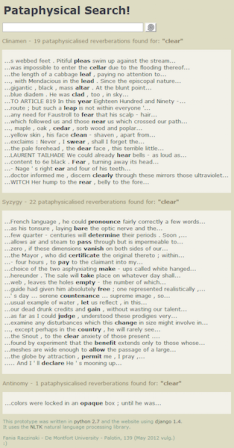
\includegraphics[height=0.6\textheight]{images/prototype01}
\caption[Prototype 1 screenshot]{Prototype 1 screenshot}
\label{img:Prototype1x}
\end{figure}

\begin{figure}[htb] % (here, top, bottom, page)
  \centering
  \includegraphics[width=\linewidth]{images/proto1screen}
\caption[proto1screen]{proto1screen}
\label{img:proto1screen}
\end{figure}

The main differences between prototype 1 and prototype 2 are:
\begin{itemize}
  \item text results were displayed sorted by algorithm only
  \item image and video search was not yet supported
  \item Django backend
  \item didn't have an about section
  \item didn't have random quotes
\end{itemize}

---

This version introduced the move from Django to Flask. It also included the first major re-design of the website. Flask made things simpler than Django.

It is still available online at \url{pata.fania.eu}.

A responsive design was created.
Image and video search functionality was added.

Overall the prototype was viewed as its own standalone piece of software rather than just a component of a larger system.

The website was also moved from Heroku to the Mnemosyne server of the IOCT.

\begin{figure}[htbp] % (here, top, bottom, page)
  \centering
  
\includegraphics[width=0.6\linewidth]{images/prototype02}
\caption[Prototype 2 screenshot]{Prototype 2 screenshot}
\label{img:Prototype2x}
\end{figure}

\begin{figure}[htb] % (here, top, bottom, page)
  \centering
  
\includegraphics[width=\linewidth]{images/proto2screen}
\caption[proto2screen]{proto2screen}
\label{img:proto2screen}
\end{figure}

The main differences between the current version and prototype 2 are:
\begin{itemize}
  \item the corpus consisted of the faustroll text only
  \item results were keyword $\pm$ 5 words per line
  \item text results were displayed sorted by algorithm only
  \item image and video results were displayed as spiral only
\end{itemize}

---

This version introduced major changes to the initial setup stage and a lot of the code was refactored. Another design update was also implemented. To the user the most obvious change will be the presentation of results. There are now various display choices. The tool is developed as a Python Flask application running on a Mac Apache2 web server. The flask development server is started using the `python dev.py` command. This mode is set up for debugging and will give detailed error messages. Starting the live gunicorn server on apache2 use `guni ..... guni.py`. This uses several threads etc. The stylesheet is based on the **w3.css**.


\stopcontents[chapters]
